\chapter{Lecture 28 - Solving Boundary value Problems Using the Shooting Method}
\label{ch:lec28n}
\section{Objectives}
The objectives of this lecture are to:
\begin{itemize}
\item Review basic concepts for Boundary Value Problems with a single independent variable.
\item Describe the Shooting Method.
\item Do an example problem.
\end{itemize}
\setcounter{lstannotation}{0}

\section{Boundary Value Problems}
A boundary value problem (BVP) consists of a governing equation and boundary conditions.  For a second-order boundary value problem with one spatial dimension\sidenote{Here we assume that the independent variable is a \emph{spatial} variable.  This is the conventional approach for applications of interest for this class.}, the general form of the governing equation is given in Equation \ref{eq:lec28n-bvp-gov-eq}:
\begin{equation}
\frac{d^2 u}{dx^2} = f\left(x,u,\frac{du}{dx}\right), \ \ a\le x \le b
\label{eq:lec28n-bvp-gov-eq}
\end{equation}
where it is understood that $a<b$.  

In order to obtain a unique solution, suitable boundary conditions must be provided.  Linear boundary conditions for the second-order problem take the form shown below:
\begin{align*}
A_1u(a)+B_1u^{\prime}(a)&=C_1 \\
A_2u(b)+B_2u^{\prime}(b)&=C_2
\end{align*}
where $A_i$, $B_i$, and $C_i$ are constants and are not \emph{all} zero for any value of $i$.

\newthought{Knowing what constitutes} a \emph{suitable} set of boundary conditions is part of your job as an engineer.  Depending on the given boundary conditions, the BVP may have one unique solution, no solution, or infinitely many solutions. Somtimes it is hard to tell in advance which of these will turn out to be the case.  Physical insight and intuition can play an important role in predicting these outcomes so it is essential that one understands the physical interpretation of a proposed set of boundary conditions.

There are three basic types of boundary conditions:\marginnote{\textbf{Note:}This classification scheme is also discussed in Lecture 22 of the Analytical Methods portion of this text.}
\begin{itemize}
\item \textbf{Type 1} or \emph{Dirichlet} boundary conditions.  For this type of boundary condition, the value of the dependent variable is directly fixed on the boundary.  For example:
\begin{equation*}
u(a) = 100
\end{equation*}
For a BVP related to the heat equation, for instance, this is equivalent to specifying the temperature on a boundary.
\item \textbf{Type 2} or \emph{Neumann}\sidenote{Here we refer to Carl Gottfried Neumann who was a German mathematician in the late 19th and early 20th century.  He taught at several universities and carried out research in pure and applied mathematics.  There are several other mathematical terms named after him including the Neumann series, the Neumann boundary value problem and the Neumann-Poincar\'e operator.  } boundary conditions.  For this type of boundary condition, the derivative of the dependent variable is directly fixed on the boundary.  For example:
\begin{equation*}
\frac{du}{dx}\Bigl|_{x=b} = 0
\end{equation*}
For a BVP related to the heat equation where the dependent variable is temperature, this is equivalent to specifying the heat flux on a boundary.  For the example given, if we set the heat flux equal to zero, that is interpreted as an \emph{insulated} boundary condtion.

\item \textbf{Type 3} or \emph{Robin}\sidenote{Named for Victor Gustave Robin who was a French matematician who lectured at the Sorbonne in Paris. To the best of this author's knowledge, he was not associated in any way with Batman.} or just \emph{mixed} boundary conditions. As the reader may have deduced by now, boundary conditions of this type involve both the dependent variable and its derivative.  For example:
\begin{equation*}
\frac{du}{dx}\Bigl|_{x=a} = -h\left(u(a) - T_{\text{env}}\right)
\end{equation*} 
where $T_{\text{env}}$ refers to the environmental temperature near the boundary and $h$ is a non-negative constant. This example corresponds to heat transfer by convection.  The constant $h$ is the convective heat transfer coefficient and relates heat flux at the boundary to the difference between the temperature at the boundary of the domain ($u(a)$) and $T_{\text{env}}$.  If $h$ is high then a large heat flux can be passed through the boundary with only a small temperature difference; if $h$ is low then the surface temperature must be much higher than the surrounding environment to transmit significant amounts of heat.  In the limit of $h\to 0$, the boundary becomes insulated.

\end{itemize}

\section{The Shooting Method}
We will introduce and illustrate our first method for solving BVPs, the shooting method, with an example.

\vspace{0.25cm}

\noindent\textbf{Problem Statement:}

\vspace{0.1cm}

\noindent A pin fin is a slender extension attached to increase the surface area and enable greater heat transfer.  When convection and radiation are included in the analysis, the steady-state temperature distribution, $T(x)$, along a pin fin can be caluclated from the solution of the equation below:
\begin{equation}
\frac{d^2T}{dx^2} - \frac{h_cP}{kA_c}\left(T - T_s\right)-\frac{\epsilon \sigma_{SB}P}{k A_c}\left(T^4 - T_s^4 \right) = 0, \ \ 0 \le x \le 0.1
\end{equation}
with boundary conditions $T(0)=T_A$ and $T(0.1)=T_B$.  A schematic of the system is shown in Figure \ref{fig:lec28n-ex1-schematic}.  There are a number of parameters given in the equation.  These are specified in Table \ref{tab:lec28n-ex1-parameters}.
\begin{marginfigure}[-4.5cm]
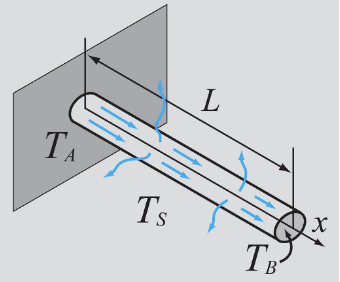
\includegraphics{lec28n-ex1-schematic.png}
\caption{Pin Fin Boundary Value Problem Schematic.}
\label{fig:lec28n-ex1-schematic}
\end{marginfigure}

\begin{table}
\begin{tabular}{|c|c|}
\hline
\textbf{Parameter} & \textbf{Value} \\ \hline
Convective heat transfer coefficient ($h_c$) & 40 $\text{W}/\text{m}^2\text{-K}$ \\ \hline
Perimeter of the pin ($P$) & 0.016 m \\ \hline
Radiative emissivity of the surface ($\epsilon$) & 0.4 \\ \hline
Thermal conductivity of the pin material ($k$) & 240 $\text{W}/\text{m-K}$ \\ \hline
Cross-sectional area of the fin ($A_c$) & $1.6 \times 10^{-5} \text{m}^2$ \\ \hline
Temperature of surrounding air ($T_S$) & 293 K \\ \hline
Stefan-Boltzmann constant ($\sigma_{SB}$) & $5.67 \times 10^{-8} \text{W}/\text{m}^2\text{-K}^4$ \\ \hline
Temperature of fin at base ($T_A$) & 473 K \\ \hline
Temperature of fin at end ($T_B$) & 293 K \\ \hline
\end{tabular}
\caption{Example problem parameters.}
\label{tab:lec28n-ex1-parameters}
\end{table}

\newthought{It is worth} taking a moment to classify the given problem.  This is a 2\textsuperscript{nd}-order, non-homogeneous, non-linear, boundary value problem with non-homogeneous type-1 boundary conditions.  Since it is non-linear and also not separable, none of the analytical methods we learned in the first portion of this book are applicable.  We need to solve the problem numerically.  Since we just finished a long section describing numerical methods for initial value problems, maybe there is a way we can use one those tools---like an explicit Runge-Kutta method---to solve this problem.  With the Shooting method, we do exactly that.

\subsection{Algorithm}
\begin{enumerate}
\item \textbf{Formulate your BVP as an IVP.}  Here we will introduce a new dependent variable, $w$:

\begin{align*}
w &= \bracketVectorstack{T \\ T^{\prime} }, \ \ w(0) = \bracketVectorstack{T_A \\ T^{\prime}_A} \\
dw &= \bracketVectorstack{T^{\prime} \\ T^{\prime \prime}} \\
 &= \bracketVectorstack{w(2) \\ \frac{h_c P}{kA_c}\left(w(1)-T_s\right) + \frac{\epsilon \sigma_{\text{SB}}P}{kA_c}\left(w(1)^{4} - T_s^4 \right)}
\end{align*}
\marginnote[-5.5cm]{\textbf{Note:} the ``initial'' condition $T^{\prime}_A$ is not part of the given boundary value problem.  We will deal with that in the next step.}

\begin{marginfigure}
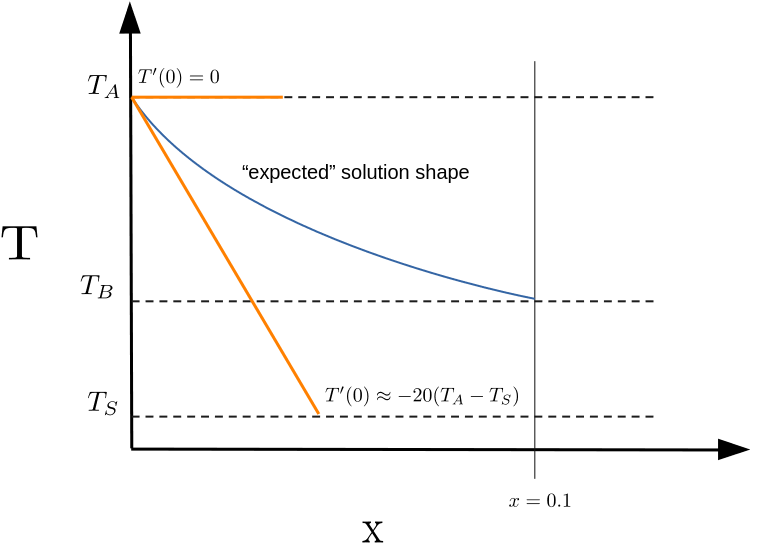
\includegraphics{lec28n-ex1-slope-est.png}
\caption{Notional pin temperature profile.}
\label{fig:lec28n-ex1-slope-est}
\end{marginfigure}

\item \textbf{Provide an estimate of the initial values.} We re-expressed our BVP as an IVP.  The problem is, of course, that the BVP specifies the temperature at $x=1$, but not the slope of the temperature at $x=0$ that we use in the IVP statement.  From the physics of the problem, we expect that $T^{\prime}(0)$ will be \emph{negative}.  The whole point of the pin fin is to draw energy from whatever it is attached to (at $x=0$) and transfer it by convection to the environment; this will result in a negative temperature gradient at the root of the fin.  What we do \emph{\textbf{not}} know is the actual value of $T^{\prime}(0)$ that will result, upon solving the IVP, in the temperature at the tip of the fin being equal to the boundary condition specified in the BVP, $T(0.1)=T_B$.  So we pick an informed estimate of $T^{\prime}(0)$.\sidenote{If we adopt the logical ``firearms analogy'' for the shooting method, think of this step as \emph{taking aim.}}

\item \textbf{Solve the IVP using your method of choice.}  We have introduced several: Euler's method, Midpoint method, any kind of Runge-Kutta method whether a method built in to MATLAB or something you wrote yourself.\sidenote{Continuing in the analogy, this is where you take your shot.  If it makes the whole affair any less tedious, you might imagine a squad of storm troopers with their blasters chasing rebel scum through the corridors of the Death Star: \emph{``pew, pew, pew...''}}

\item \textbf{Evaluate $T(b)$ and compare with $T_B$}.  If our aim was true, we would ``hit'' $T(b)=T_B$ with our ``shot.''  In MATLAB you might do this as follows:

\begin{enumerate}
\item Define a function that takes the estimate for $T^{\prime}(0)$ as an argument and retuns the resulting value of $T(b)$.
\item Create a second function that returns the difference between the function described above, and $T_B$.  For example:
\begin{lstlisting}[style=myMatlab]
tgt_err_fun = @(dTa) fun(dTa) - Tb
\end{lstlisting}
where \lstinline[style=myMatlab]{dTa} is the estimated value for $T^{\prime}(0)$, \lstinline[style=myMatlab]{fun} is the aforementioned function, and \lstinline[style=myMatlab]{Tb} is $T_B$.
\end{enumerate}

\item \textbf{Iteratively repeat steps 2-4 until all boundary conditions are satisfied}.  In this case, we iterate until $T(0.1) = T_B$. If we adopt the approach introduced in step 4, we can use one of the several algorithms for solving non-linear equations that we studied earlier in this class.\sidenote{Noting that the bisection and secant methods each require two estimates for $T^{\prime}(0)$ and further, for the bisection method, the two slope estimates must bracket the value of $T^{\prime}(0)$ that results in $T(0.1)=T_B$.}   

\end{enumerate}


\begin{lstlisting}[style=myMatlab,name=lec28n-ex1]
%% Lecture 28 - Solving BVPs with the Shooting Method
clear
clc
close 'all'
%% Define the ODE and all parameters
a = 0; b = 0.1;
Ta = 473; % K, temperature at base of fin
Tb = 293; % K, temperature at the tip of the fin
N = 1000; %
ode = @(x,T) pin_fin(x,T); /*!\annotation{lst:ann28n-1}!*/
\end{lstlisting}

\marginnote[-0.25cm]{

\noindent \ref{lst:ann28n-1} The governing equation is implemented as a local function and will be provided at the end of the script.

}

\marginnote[0.5cm]{

\noindent \ref{lst:ann28n-2} For this example we will use our own implementation of the classical 4\textsuperscript{th}-order Runge Kutta method.  As an alternative we could use one of MATLAB's built-in methods.  

}
\begin{lstlisting}[style=myMatlab,name=lec28n-ex1]
%% set RK4 solver tableau parameters
% note: any other ODE solver would also suffice.
solver = @odesExplicitRK; /*!\annotation{lst:ann28n-2}!*/
s = 4;
BT = zeros(s+1,s+1); % Butcher Tableau for RK method
C = [0; 1/2; 1/2; 1; 0]; % sample points
B = [0 1/6 2/6 2/6 1/6]; % weights
A = [0 0 0 0;    % RK matrix
    1/2 0 0 0;
    0 1/2 0 0;
    0 0 1 0;];
BT(:,1) = C;
BT(end,:) = B;
BT(1:s,2:end) = A;
\end{lstlisting}

\marginnote{

\noindent \ref{lst:ann28n-3} Here we define a function that will take the ODE, a solve, and a guessed value for the initial conditions as needed for the shooting method.

\vspace{0.1cm}

\noindent \ref{lst:ann28n-4} We also need to define a function that will solve the ODE with the guessed value and return 0 when the ``correct'' value is guessed.  As written, this function can thus be passed to any root-finding algorithm.

}
\begin{lstlisting}[style=myMatlab,name=lec28n-ex1]
%% Commence Shooting Method
odeWithSolver = @(dTa_g) solver(ode,a,b,N,[Ta;dTa_g],BT); /*!\annotation{lst:ann28n-3}!*/

tgt_err_fun = @(dTa_g) shot_function(odeWithSolver,dTa_g) 
                                                   - Tb; /*!\annotation{lst:ann28n-4}!*/
\end{lstlisting}

Since some of the root-finding methods that we can choose from require two estiimates of the slope and, for bisection method, the estimates must bracket the actual slope, we will propose a ``high'' and ``low'' estimate for the initial slope.
\begin{lstlisting}[style=myMatlab,name=lec28n-ex1]
% need two guesses at the slope
dT_a_H = 0; % slope = 0 at x=a means no heat transfer out.
dT_a_L = 4*(Tb - Ta)/(b-a); % guess a strong linear function
\end{lstlisting}

For this demo, I like to choose from among several available algorithms for solving nonlinear equations.  The functions \lstinline[style=myMatlab]{BisectionRoot} and \lstinline[style=myMatlab]{SecantRoot} are unchanged from when they were introduced earlier in the course.

Note that when this block of code is complete, we will have solved for the value of $T^{\prime}(0)$---denoted \lstinline[style=myMatlab]{dT_a}---that results in $T(0.1)=T_B$.

\begin{lstlisting}[style=myMatlab,name=lec28n-ex1]
method = 4;
switch method
    case 1
        tol = 1e-4; % tolerance on convergence to the BC
        dT_a = BisectionRoot(tgt_err_fun,dT_a_H,dT_a_L,tol);
    case 2
        tol = 1e-4; % tolerance on convergence to the BC
        imax = 100;
        dT_a = SecantRoot(tgt_err_fun,dT_a_H,dT_a_L,tol,imax);
        
    case 3
        dT_a = fzero(tgt_err_fun,dT_a_H);
        
    case 4
        dT_a = fsolve(tgt_err_fun,dT_a_H);
        
    otherwise
        error('Invalid Solver Choice!');
end
\end{lstlisting}
Now we should visualize the result.  
\begin{lstlisting}[style=myMatlab,name=lec28n-ex1]
%% Solve one last time with converged dT_a
T = odeWithSolver(dT_a);

x = linspace(a,b,N);
figure(1)
plot(x,T(1,:),'-b','linewidth',3);
title('Pin Fin Temperature Profile',...
    'fontsize',14,'fontweight','bold');
xlabel('X [m]','fontsize',12,'fontweight','bold');
ylabel('T [^\circ C]','fontsize',12,'fontweight','bold');
grid on
set(gca,'fontsize',10,'fontweight','bold');
\end{lstlisting}
\begin{marginfigure}
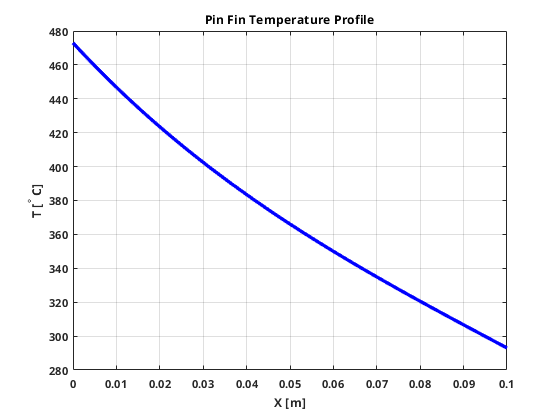
\includegraphics{lec28n-ex1-sol.png}
\caption{Shooting Method Example Solution.}
\label{fig:lec28n-ex1-sol}
\end{marginfigure}

The resulting temperature profile through the pin fin is shown in Figure \ref{fig:lec28n-ex1-sol}.  

\marginnote{

\vspace{0.25cm}

\noindent\textbf{Note:} Take a few moments to think about this figure.  Does the shape match your expecation?  How do you think the shape of the curve would change if $h_c$ were much larger or smaller?  Readers are strongly encouraged to solve this problem and test these hypotheses. 

\vspace{0.25cm}

\noindent It is not against the law also to critically consider the given boundary conditions.  How realistic is it to specify the temperatures at both ends of the pin fin?  What aspects of the solution should you look at to evaluate the \emph{performance} of the pin fin as a heat management device?
}

Local functions defined above are included here.  %The functions \lstinline[style=myMatlab]{odesExplicit}, \lstinline[style=myMatlab]{SecantRoot}, and \lstinline[style=myMatlab]{BisectionRoot} are not shown in this listing for the sake of brevity.
\begin{lstlisting}[style=myMatlab,name=lec28n-ex1]
%% Local Functions
function Tb = shot_function(odeWithSolver,dT_a)
% given an estimate for T'(a), solves the IVP and returns
% the value of T(b).
T_trial = odeWithSolver(dT_a);
Tb = T_trial(1,end);
end

function F = pin_fin(~,T)
% define the IVP
% two args so it can work with ode45
Ac = 1.6e-5; % m^2, fin cross sectional area
P = 0.016; % m, perimeter of pin cross section
h_c = 40; % W/m^2-K, convective heat transfer coefficient of air
k = 250; % W/m-K, thermal conductivity of pin material
emiss = 0.5; % emissivity of pin material
sigma_sb = 5.67e-8; % W/m^2-K^4, Stefan-Boltzmann constant
Ts = 293; % K, temperature of surrounding air

F = nan(2,1);
F(1) = T(2);
F(2) = ((h_c*P)/(k*Ac))*(T(1) - Ts) + ...
    ((emiss*sigma_sb*P)/(k*Ac))*(T(1).^4 - Ts^4);

end

function y = odesExplicitRK(ODE,a,b,N,yINI,BT)
% function y = odeExplicitRK(ODE,a,b,h,yINI,BT)
% y = solution (vector)
% ODE = function handle for y'
% a,b = begining and end of the interval for solution
% N = number of steps between a and b
% yINI = initial value for the solution
% BT = Butcher Tableau

% get Butcher Tableau Parameters
s = length(BT)-1;
c = BT(1:s,1);
B = BT(s+1,2:end);
A = BT(1:s,2:end);
stages = s;

x = linspace(a,b,N);
sys_size = length(yINI);
y = nan(sys_size,N);
y(:,1) = yINI;
h = x(2)-x(1);
for t = 1:(N-1)
    Xi = nan(sys_size,stages);
    
    for s = 1:stages
       Xi(:,s) = y(:,t);
       for i = 1:(s-1)
          Xi(:,s) = Xi(:,s) + h*A(s,i)*ODE(x(t)+c(i)*h,Xi(:,i)); 
       end
    end
    
    y(:,t+1) = y(:,t);
    for i = 1:stages
       y(:,t+1) = y(:,t+1) + h*B(i)*ODE(x(t)+c(i)*h,Xi(:,i)); 
    end
    
end
end

function x_bi = BisectionRoot(fun,a,b,TOL)

tol = TOL;
x_bi = (a+b)/2;
% verify that fun(a) and fun(b) have different sign
if(fun(a)*fun(b)>0)
   error('No root lies between %g and %g!\n',a,b); 
end

maxIt = 1e2;
for k = 1:maxIt
    FxNS = fun(x_bi);
    
    % check if FxNS is within the tolerance
    if (abs(FxNS) < tol)
        return;
    end
    
    % update brackets
    if (fun(a)*FxNS < 0)
        b = x_bi;
    else
        a = x_bi;
    end
    
    % update estimated x_bi based on new bracket
    x_bi = (a+b)/2;
       
end

% if I ever get here, then I failed to meet the tolerance 
% within the maximum number of iterations
fprintf('Warning: failed to find root within specified tolerance.\n');
fprintf('Current root: %g, fun(x_bi) = %g. \n',x_bi,fun(x_bi));


end

function Xs = SecantRoot(Fun,Xa,Xb,Err,imax)

for i = 1:imax
   FXb = Fun(Xb);
   Xi = Xb - FXb*(Xa - Xb)/(Fun(Xa) - FXb);
   
   if abs((Xi - Xb)/Xb) < Err
       Xs = Xi;
       break;
   end
   Xa = Xb;
   Xb = Xi;
     
        
end

end

\end{lstlisting}

